\section{Background}
%OR: \section{Tools and Methods}
\label{sec:background}

The background's depth and breadth depend on the depth needed to understand your project.
It is not a place to just write about everything you know that is vaguely connected to your project. 
The theory is here to help the readers that do not know the theoretical basis of your work, so that they 
can gain sufficient understanding to understand your contributions. In particular, the theory section provides 
an opportunity to introduce terminology that can later be used without disturbing the text with a definition.  

When introducing techniques or results, always reference the source. 
Be careful to reference the original contributor of a technique and not just someone who happens to use the technique.%
\footnote{But always make sure that you have read the work you are citing --- if not, cite someone who has!}
For results relevant to your work, 
you would want to look particularly at newer results so that you have referenced the most up-to-date work in your area. 
If you do not have the source handy when writing, mark in the text that a reference is needed and add it later. \todo{add reference} 
Web pages are not reliable sources --- they might be there one day and removed the next; and thus should be avoided, if possible. 
A verbal discussion is not a source and should normally not be referenced.  
The bulk of citations in the report will appear in Section~\ref{sec:related_work}. 
However, you will often need to introduce some terminology and key citations already in this section. 
%
You can cite a paper in the following manner (and several other versions, 
see the \verb!natbib! package documentation):

\begin{itemize}
\item when referring to authors:\\
 \citet{Authorson;Bobsen:10} stated something rather nice.
\item to cite indirectly: \\
 Papers should be written nicely \citep{Authorson;Bobsen:10}
{\em or\/}\\
In \cite{Authorson;Bobsen:10}, a less detailed template was presented.
\item To just cite the authors: \\
\citeauthor{Authorson;Bobsen:10} wrote a nice paper.
Or just the year: \citeyear{Authorson;Bobsen:10}.
\item You can even cite specific pages: \citet[p. 3]{Authorson;Bobsen:10}.
\end{itemize}

You should obviously always cite your teacher's work \citep{BenyonEA:13}, 
even if it is completely irrelevant \citep{Das;Gamback:13a} or very old \citep{AlshawiEA:91b}.
Digging up an even older book can also appear impressive \citep{Diderichsen:57}.
(Or? ;-)

\subsection{Introducing Figures}

\begin{figure}[t!]
\centering
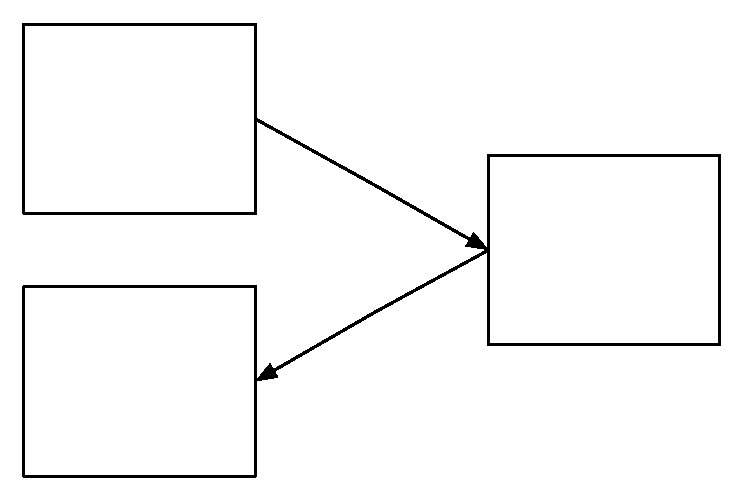
\includegraphics[width=0.5\columnwidth]{figs/figure1.pdf}
\caption[Boxes and arrows are nice]{Boxes and arrows are nice (adapted from \citealp{Authorson;Bobsen:10}, with permission)}
\label{fig:BoxesAndArrowsAreNice}
\end{figure}

Remember that when you borrow figures you should always credit the original author --- such as 
Figure~\ref{fig:BoxesAndArrowsAreNice} (adapted from \citealp{Authorson;Bobsen:10}),
as well as state that you have permission to reprint it (e.g., if it is published under a Creative Commons License,
or if you have gained explicit permission from the author). 

Do not just put the figure in and leave it to the reader to try to understand what the figure is. 
The figure should be included to convey a message and you need to help the reader to understand the message 
intended by explaining the figure in the text. Hence {\bf all} figures and tables should always be referenced in the text.
There will often be specific parts of a figure or table that you want the reader to pay special attention to (and that you
discuss in more detail in the text). It is helpful if you mark those parts clearly (e.g., by circling them, pointing them out
with arrows, using different colours and fonts, etc.)

It is good practice to add a note about a missing figure in the text,
such as the completely amazing stuff that will appear in Figure~\ref{fig:AmazingFigure}.

Narrow graphics together with the single-column format may lead to large empty spaces.
If you have multiple graphics with related content, it may be preferable to combine them in one graphic.
You can identify the sub-graphics with sub-captions below the sub-graphics numbered (a), (b), (c) etc., and using 9pt text.
The \LaTeX\ packages wrapfig, subfig, subtable and/or subcaption may be useful.

\begin{figure}[t!]
\centering
\missingfigure{Here we will add an amazing figure explaining it all}
\caption{A missing figure}
\label{fig:AmazingFigure}
\end{figure}

\subsection{Introducing Tables in the Report}

\newcommand\emc{-~~~~}
\begin{table}[t!]
\centering
\caption{Example table (F$_1$-scores)}
\begin{tabular}{c|c|rrrrrr}
\tabletop
Langs                       & Source                 & \multicolumn{1}{c}{Lang1} & \multicolumn{1}{c}{Lang2} & \multicolumn{1}{c}{Univ}                                                     & \multicolumn{1}{c}{NE}    & \multicolumn{1}{c}{Mixed} & \multicolumn{1}{c}{Undef} 
\\ \tablemid
\multirow{5}{*}{EN-HI} & FB+TW                  & 54.22 & 22.00 & 19.70 & 4.00  & 0.05  & 0.03  \\
                       & FB                     & 75.61 & 4.17  & 18.00 & 2.19  & 0.02  & 0.01  \\  
                       & TW                     & 22.24 & 48.48 & 22.42 & 6.71  & 0.08  & 0.07  \\  
                       & Vyas                   & 54.67 & 45.27 & 0.06  & \emc  & \emc  & \emc  \\ 
                       & FIRE                   & 45.57 & 39.87 & 14.52 & \emc  & 0.04  & \emc  \\ \tablemid
\multirow{2}{*}{EN-BN} & TW                     & 55.00 & 23.60 & 19.04 & 2.36  & \emc  & \emc  \\ 
                        &  FIRE                 & 32.47 & 67.53 & \emc  & \emc  & \emc  & \emc  \\ \tablemid
EN-GU                  & FIRE                   & 5.01  & {\bf 94.99} & \emc  & \emc  & \emc  & \emc  \\ 
\tablemid
DU-TR                  & Nguyen                 & 41.50 & 36.98 & 21.52 & \emc  & \emc  & \emc  \\ \tablemid

EN-ES                  & \multirow{4}{*}{\rotatebox[origin=c]{90}{EMNLP}} 
                                                & 54.79 & 23.50 & 19.35                                                    & 2.08  & 0.04  & 0.24  \\ 
EN-ZH                  &                        & 69.50 & 13.95 & 5.88                                                     & 10.60 & 0.07  & \emc     \\ 
EN-NE                  &                        & 31.14 & 41.56 & 24.41                                                    & 2.73  & 0.08  & 0.08  \\ 
AR-AR                  &                        & 66.32 & 13.65 & 7.29                                                     & 11.83 & 0.01  & 0.90    \\ \tablebot
\end{tabular}
\label{tab:ExampleTable}
\end{table}

As you can see from Table~\ref{tab:ExampleTable}, tables are nice. 
However, again, you need to discuss the contents of the table in the text. 
You do not need to describe every entry, but draw the reader's attention to what is important in the table,
e.g., that $94.99$ is an amazing F$_1$-score for the English-Gujarati language pair (and that probably something fishy happened there). 
\todo[inline]{There is always some more stuff that you will need to add at some later point. 
Be sure to at least make a note about it somewhere.}
